% !TEX root = ../thesis-WW.tex

\chapter{Introduction} \label{chap:introduction}

The 3D attitude of a rigid body is a key concept in modeling our physical world.
It can be defined as the directions of the three axes of an orthogonal frame fixed to the rigid body in the inertial frame, and therefore describes the orientation of the rigid body.
The attitude is a state involved with rigid body mechanics, and is usually controlled in a robotic system through actuators to achieve the goal of alignment or moving to a specific position.
As a feedback controller also needs estimation of the state, a number of sensors are usually used to determine the attitude of the rigid body.
These sensors can usually be classified into the following categories:
(i) infrastructures that measure the attitude directly, for example an optical motion capture system;
(ii) a gyroscope that measures the angular velocity;
(iii) direction sensors that measure reference directions in the inertial frame, such as magnetometers, star trackers, etc;
(iv) sensors that measure the surrounding environment, such as various cameras, lidars, etc.

These sensors provide either direct or indirect information of the attitude of a rigid body.
But one common feature is that they are all subject to measurement noises.
The noise characteristics of different types of measurement are also different.
For example, the attitude integrated from angular velocity measured by a gyroscope suffers from accumulated integration of bias, and therefore is only accurate within a short period of time.
It is similar for a visual odometry algorithm that estimates the attitude by capturing surrounding visual features using cameras.
On the other hand, the attitude inferred from measurements of reference directions may be affected by instantaneous disturbances, but the average noise remains low for a long period of time.
Thus, it is common that different sensors are combined to get a robust attitude estimate, by leveraging their different noise characteristics.

This motivates the need to model the uncertainty of the attitude.
As when combining the estimates from two or more different measurement sources, one must decide on how much confidence should be placed on each individual source.
As a rule of thumb, the measurement with more uncertainty should play a less important role in determining the final estimation.
Consequently, a metric that describes the uncertainty for the estimated attitude is needed to weigh the measurements.
From another point of view, uncertainty of the final estimation can play an important role in decision making for a robotic system.
For example, if the uncertainty for attitude is too large, a robot may take some safety measures like slowing down, to avoid possible collisions.

This dissertation focuses on modeling the uncertainty of the rigid body attitude in a geometric awaring and global way.
More specifically, the uncertainty is formulated on the curved and compact manifold where the attitude naturally resides in a global fashion.
Furthermore, a model for the correlation between attitude and other Euclidean quantities, for example the 3D location, is proposed.
Based on these, three typical estimation problems in aerospace and robotics engineering are investigated: (i) attitude estimation with a gyroscope and direction sensors, (ii) loosely coupled IMU-GNSS integration for navigation, and (iii) visual-inertial navigation and odometry with a RGB-D camera. 

\section{Motivation and Goal}

In existing algorithms for attitude estimation from different sensors, the uncertainty of attitude is usually modeled in two different ways.
In the first way, attitude parameterizations, such as Euler angles or quaternions, are treated directly as quantities in the Euclidean space, and the Gaussian distribution is used to model their uncertainty.
This method entirely ignores the geometric constraints on the attitude parameterizations, such as the singularity of Euler angles, or that a quaternion representing attitude should have unit norm.
As a result, its accuracy is typically low, and may have numerical issues associated with singularities, or that the covariance matrix becomes singular.

Instead of directly treating the attitude parameterizations as in Euclidean space, the more popular second approach treats the 3-dimensional parameterizations of attitude \textit{error} as in Euclidean space.
In this approach, since the attitude error is typically small, it avoids the singularity of the parameterization, which is usually at 180 degrees.
Also, by using the minimal three dimensional parameterization, it avoids a equality constraint that makes the covariance matrix for a unit quaternion singular.
The parameterizations frequently used include rotation vectors and modified Rodrigues parameters.

Although the second approach of modeling attitude uncertainty seems very reasonable, and usually achieves good estimation accuracy of attitude in practical applications, it still does not faithfully respect the geometric structure of the attitude space.
For example, the space of rotation vectors is actually cyclic, i.e., any rotation vectors with the same direction that differ in length by $2k\pi$, $k\in\mathbb{Z}$, represent the same rotation.
As a consequence, a Gaussian distribution for rotation vectors needs to be \textit{wrapped}, or \textit{folded} in order to faithfully represent the uncertainty.
Namely, the densities representing the same rotation need to be added up.
An example of a wrapped Gaussian distribution in the one dimensional rotation space is shown in Fig. \ref{fig:wrapping}.
If the uncertainty is low, or the variance of the Gaussian distribution is small, the error caused by wrapping can usually be neglected.
However, for large uncertainty, as indicated in Fig. \ref{fig:wrapping}, wrapping makes the uncertainty much larger than that indicated by the original Gaussian distribution.

\begin{figure}
	\centering
	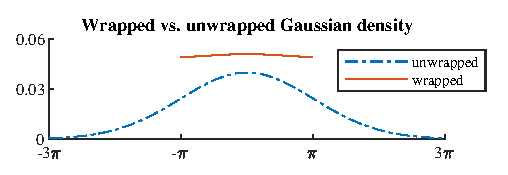
\includegraphics[scale=1.2]{figures/wrapping}
	\caption{Gaussian density vs. wrapped Gaussian density with $\mu=0$ and $\sigma^2=10$.
		The wrapped Gaussian distribution is defined in the circular space $\mathbb{R}/2\pi$ by identifying $\theta$ with $\theta+2k\pi$ for $k\in\mathbb{Z}$, so the densities beyond $[-\pi,\pi]$ are wrapped into $[-\pi,\pi]$. \label{fig:wrapping}}
\end{figure}

In this dissertation, a different approach is sought to model large uncertainty of rigid body attitude which cannot be accurately described by a Gaussian distribution as discussed above.
The key idea is that instead of treating parameterizations of attitude as quantities in Euclidean space, a probability density defined directly in the space of attitude is used.
Classic densities include the matrix Fisher distribution defined on the three dimensional special orthogonal group $\SO{3}$, and the Bingham distribution defined on the unit three sphere $\Sph^3$.
In this way, the geometric constraints on the parameterizations of attitude are completely avoided, and the densities are suitable for arbitrarily large uncertainty including a uniform distribution, which is made possible by the compactness of the attitude space.

To apply these densities in estimation problems encountered in engineering, the correlation between attitude and other Euclidean quantities must also be considered, since attitude is usually jointly estimated with these quantities, such as the gyroscope bias, and the position.
This issue is investigated in this dissertation by introducing a new probability density defined on $\SO{3} \times \mathbb{R}^n$, referred to as the matrix Fisher--Gaussian (MFG) distribution.
With this new tool, classic estimation problems in engineering, including attitude determination and localization, can be tackled with probabilistic models that fully respect the underlying geometric structure of the attitude space.
Therefore, in the presence of large uncertainty, for example unknown initial conditions, estimators can converge with a much faster speed than the conventional Gaussian approach, thanks to the accurate modeling of large uncertainty.

\section{Literature Review}

Probabilistic models that describe uncertainty on curved manifolds have been studied by statisticians in the branch called \textit{directional statistics}.
In this section, the developments in directional statistics that are relevant to this dissertation are reviewed.
Then, classic methods for rigid body estimation using gyroscopes and direction sensors are introduced.
Moreover, some attempts in applying the matrix Fisher distribution, and Bingham distribution to attitude estimation are examined.
Finally, the progresses in rigid body pose estimation (attitude and position) using various cameras with an IMU (inertial measurement unit), are reviewed.

\subsection{Directional Statistics} \label{section:intro-review-direction}

Although the Gaussian distribution is the dominate probabilistic model in both theoretical research and practical engineering, it falls short when the data of interest are on curved manifold, such as the unit sphere $\Sph^2$, and the special orthogonal group $\SO{3}$.
Statisticians have proposed new models directly defined on these manifold, to replace the Gaussian distribution when the uncertainty of data is large.
The materials in this subsection are mostly based on the book \cite{mardia2009directional}.
Another useful exposition of models on the Stiefel and Grassmann manifolds can be found in \cite{chikuse2003statistics}.

\paragraph{Models on Unit Circle and Sphere}

One of the most frequently encountered and simplest manifold is the one dimensional unit circle: $\Sph^1 = \{ x\in\mathbb{R}^2 \,|\, \norm{x} = 1 \}$.
Any element on the unit circle can be written as an angle $\theta\in\mathbb{R}$, however, $\theta$ and $\theta+2k\pi, k\in\mathbb{Z}$ represent the same element due to the cyclic nature of $\Sph^1$.
As a consequence, the unit circle can also be regarded as the space of one dimensional rotation, i.e., the two dimensional special orthogonal group $\SO{2} = \{ R\in\mathbb{R}^{2\times 2} \,|\, RR^T = I_{2\times 2},\, \det R = 1\}$, where
\begin{align*}
	R = \begin{bmatrix}
		\cos\theta & -\sin\theta \\
		\sin\theta & \cos\theta
	\end{bmatrix}.
\end{align*}
Various probability densities have been developed on $\Sph^1$, such as the von Mises distribution \cite{von1918uber}, wrapped normal (Gaussian) distribution, wrapped Cauchy distribution, projected normal distribution (angular Gaussian distribution), etc.
The first three distributions are uni-modal and have similar shapes (see \cite[Figure 3.3]{mardia2009directional}), whereas the last can be bi-modal.
Among these, the von Mises distribution is one of the most frequently used models, and can be regarded as an analog of Gaussian distribution on $\Sph^1$, due to their several similarities.

The von Mises distribution can be generalized into (hyper) unit spheres $\Sph^n = \{ x\in\mathbb{R}^{n+1} \,|\, \norm{x}=1 \}$, for $n\geq 2$, and is usually named as von Mises--Fisher distribution \cite{fisher1953dispersion}.
If $x\in\Sph^n$ follows a von Mises--Fisher distribution, it has the following density function
\begin{align*}
	p(x) = \left(\frac{\kappa}{2}\right)^{(n+1)/2-1} \frac{1}{\Gamma((n+1)/2) I_{(n+1)/2-1}(\kappa)} \expb{\kappa\mu^T x}
\end{align*}
with respect to the uniform distribution, where $\mu\in\Sph^n$, $\kappa>0$ are the parameters of the distribution, $\Gamma$ is the gamma function, $I_\nu$ is the modified Bessel function of the first kind with order $\nu$.
For the unit sphere $\Sph^2$, the density function reduces to
\begin{align}
	p(x) = \frac{\kappa}{\sinh\kappa} \expb{\kappa\mu^T x}.
\end{align}
This distribution is denoted by $x\sim \mathcal{VM}(\mu,\kappa)$.
The parameter $\mu$ represents the mean direction, and $\kappa$ represents the concentration, with larger $\kappa$ meaning higher concentration.
The von Mises--Fisher distribution is used to model the uncertainty of direction measurements in this dissertation.

\paragraph{Models on $\SO{3}$}

Another frequently encountered manifold in engineering and material science is the space of 3D rotations, i.e., the three dimensional special orthogonal group: $\SO{3} = \{ R\in\mathbb{R}^{3\times 3} \,|\, RR^T = I_{3\times 3}, \, \det R = 1\}$.
One of the most famous models on $\SO{3}$ is the matrix Fisher distribution \cite{downs1972orientation,khatri1977mises}, which is originally defined on the Stiefel manifolds, i.e., an orthogonal $r$ frame in $\mathbb{R}^n$ with $r\leq n$.
When $r=2$, $n=3$, the Stiefel manifold is $\SO{3}$ \cite[Chapter 13.2.1]{mardia2009directional}.
Similar to von Mises distribution, the matrix Fisher distribution can be regarded as an analog of Gaussian distribution on $\SO{3}$.

Any 3D rotation can also be parameterized by a unit quaternion $q\in\Sph^3$.
The space of unit quaternions $\Sph^3$ forms a double cover of $\SO{3}$, therefore, $q$ and $-q$ represent the same 3D rotation.
The Bingham distribution \cite{bingham1974antipodally} is formulated on $\Sph^n$, $n\geq 1$ with antipodal symmetry, i.e., the densities for $x$ and $-x$ are identical.
Thus, the Bingham distribution on $\Sph^3$ can be treated as a probability distribution on $\SO{3}$.
In fact, it has been shown to be equivalent to the matrix Fisher distribution on $\SO{3}$ \cite{prentice1986orientation}.
The definition, construction, and properties of these two distributions will be introduced in detail in Chapter \ref{chap:MF}.

Besides these two popular models, a ``normal'' like distribution on $\SO{3}$ is proposed in \cite{nikolayev1997normal} using the central limit theorem,
the Cayley distribution is introduced in \cite{leon2006statistical} using the Cayley transform,
and some other density functions are formulated in \cite{bunge2013texture,matthies1982form}.
These (including the matrix Fisher distribution) are further summarized under a generic approach of constructing probability distributions on $\SO{3}$ proposed in \cite{qiu2014wrapped} based on the exponential map, called the UARS model.
Moreover, the authors in \cite{qiu2014wrapped} introduced the wrapped tri-variate normal distribution on $\SO{3}$, generalizing the wrapped normal distribution on $\Sph^1$ by assuming the rotation vector follows a Gaussian distribution.

\paragraph{Correlations with Euclidean Space}

In practical applications, data on manifolds are usually coupled with other data in the Euclidean space, such as the attitude and position of a rigid body.
Therefore it is also necessary to model the correlation between the manifold and Euclidean space.
In \cite{mardia1978model}, the von Mises distribution on $\Sph^1$ and the Gaussian distribution on $\mathbb{R}^1$ are coupled to define a density on the cylinder $\Sph^1 \times \mathbb{R}^1$, where some other models \cite{abe2017tractable,johnson1978some,kato2008dependent} have also been introduced to model the correlation between $\Sph^1$ and $\mathbb{R}^1$.
In addition, the von Mises distribution has also been generalized to multi-variate von Mises distribution \cite{mardia2008multivariate} to model the correlation between pairs of several random angles in $\Sph^1$.

There have also been two attempts to couple $\SO{3}$ and $\mathbb{R}^n$.
In \cite{markley2006attitude}, the matrix Fisher distribution is coupled with the Gaussian distribution by making the parameter of the matrix Fisher part dependent on the random variable in the Euclidean space.
The same approach has also been used to couple the Bingham distribution and Gaussian distribution \cite{darling2016uncertainty}.
However, this coupling technique, although being reasonable, is not originated from a generic geometric construction principle.
As a consequence, these models require very difficult computations when applied to practical problems, especially numerical optimizations are required when performing maximum likelihood estimation, i.e., recovering parameters from data, which limits their applications.

\subsection{State Estimation on $\SO{3}$} \label{section:intro-review-estimation}

Rigid body attitude estimation is the basic algorithm for numerous robotics and aerospace applications, and has been studied extensively by researchers and practitioners.
For example, in inertial navigation, the acceleration measurement must be first transformed into the inertial frame, which requires the attitude of the accelerometer to be estimated.
For a bipedal robot, its inclination must be first estimated so that the controller can prevent it from falling.
For a telescope operating in space, such as the Hubble telescope, its attitude must be known to direct its lens to a specific area of space.

Attitude estimation algorithms can be divided into the following three categories:
(i) deterministic observers with guaranteed convergence;
(ii) nonlinear Kalman filter based stochastic filters;
and (iii) stochastic filters based on the matrix Fisher and Bingham distributions.
But before reviewing these three categories, attitude parameterizations must be first introduced.

\paragraph{Attitude Parameterizations}

The attitude of a rigid body has three degrees of freedom, however, a rotation matrix $R\in\SO{3}$ has 9 parameters, and is therefore subject to 6 equality constraints.
Due to its redundancy, few stochastic filters directly operate on rotation matrices.
Instead, people seek for attitude representations with fewer parameters.
A comprehensive review on this topic is given in \cite{shuster1993survey}.
Nevertheless, it should be noted that it is topologically impossible to have a global 3-dimensional parameterization without singular points for $\SO{3}$ \cite{stuelpnagel1964parametrization}.
Moreover, 5 is the minimum dimension to represent $\SO{3}$ in a one-to-one and global fashion \cite{stuelpnagel1964parametrization}.

Perhaps the most popular 3-dimensional parameterization of attitude is Euler angles.
The Euler angles have 24 different forms depending on the sequence of rotations, and in which frame the rotations are formulated (intrinsic and extrinsic).
The intrinsic z-y-x Euler angles are usually used in aerospace engineering, which are also referred to as the yaw, pitch and roll angles.
The singular point for this set of Euler angles is when the pitch angle is 90 degrees, which is famously known as the gimbal lock.

Another frequently used 3-dimensional parameterization is the rotation vector.
By the Euler's rotation theorem, any 3D rotation can be described by rotating about an axis $n\in\Sph^2$ by an angle $\theta\in\mathbb{R}$.
And the rotation vector is simply $v = \theta n \in \mathbb{R}^3$.
The singular point for rotation vectors is when $\norm{v} = \theta = \pi$, i.e., when the rotation angle is 180 degrees.
Two other 3-dimensional parameterizations that are used in aerospace engineering are Rodrigues parameters and modified Rodrigues parameters, given by $\rho = \tan(\theta/2) n \in \mathbb{R}^3$, and $p = \tan(\theta/4) n \in \mathbb{R}^n$, respectively.
The singular points for these two parameterizations are when $\theta = \pi$, and $\theta = 2\pi$, respectively.

As mentioned in Section \ref{section:intro-review-direction}, the attitude can also be parameterized using unit quaternions in $\Sph^3$.
This is a 4-dimensional singularity free parameterization, and is widely used in attitude estimation algorithms.
The unit quaternion corresponding to the rotation $(n,\theta)$ can be written as
\begin{align} \label{eqn:rv2qua}
	q = \begin{bmatrix} \cos(\theta/2) \\ \sin(\theta/2) n \end{bmatrix} \in \Sph^3
\end{align}
in Hamilton convention.
It should be noted that $q$ and $-q$ represent the same 3D rotation.

\paragraph{Deterministic Observers}

This type of attitude estimators assume all measurements are noise free, so the convergence from a wrong initial attitude to the true attitude can be proved using a rigorous Lyapunov argument.
Typically it is assumed that the angular velocity is measured by a gyroscope, so that the attitude can be integrated forward in time.
Also, various reference directions in the inertial frame are measured in the reference frame fixed to the rigid body (body-fixed frame), to correct the initial and integration errors.

The first and most famous attitude observer with guaranteed convergence is proposed in \cite{mahony2008nonlinear}.
This observer has been extensively used in attitude controllers for unmanned aerial vehicles.
Later, it has been generalized to deal with reference directions that are time varying in the inertial frame \cite{batista2012ges,grip2011attitude,trumpf2012analysis}.
Also, a hybrid correction scheme has been proposed in \cite{wu2015globally} to deal with the zero measure set where the initial attitude does not converge for the observer in \cite{mahony2008nonlinear}.
Moreover, the rotation of the Earth has also been incorporated to enhance attitude observability when only a single reference direction is available \cite{reis2018nonlinear}.

\paragraph{Nonlinear Kalman Filters}

Different from deterministic observers, stochastic filters assume that both the gyroscope and direction measurements are subject to noises.
And the filter determines how many weights are given to the integrated attitude and the direction measurements, based on their respective covariance matrices.
Compared to deterministic observers, filters typically have faster convergence rate when the initial uncertainty, and sensor noise characteristics are known.
On the other hand, due to the difficulty of formulating stability under stochastic settings \cite{karvonen2020stability}, convergence properties are usually not studied for stochastic filters.

A comprehensive review of attitude estimation algorithms based on extended Kalman filters (EKF) and unscented Kalman filters (UKF) has been presented in \cite{crassidis2007survey}.
The EKF can be naturally applied to attitude kinematics formulated in Euler angles \cite{farrell1970attitude,foxlin1996inertial}, Rodrigues parameters \cite{idan1996estimation}, and modified Rodrigues parameters \cite{crassidis1996attitude}.
However, due to the singularity of 3-dimensional attitude parameterizations, these filters must be operated in a limited range of attitude, which cannot undergo continuous spinning.
Also, a less noticed problem is that the Lebesgue measure in $\mathbb{R}^3$ for these parameterizations does not correspond to a uniform measure on $\SO{3}$, which means that the Gaussian distribution in $\mathbb{R}^3$ is no longer Gaussian shaped on $\SO{3}$, and this causes inaccuracy in modeling the uncertainty.

The problem caused by singularity is avoided by the celebrated multiplicative EKF (MEKF) \cite{lefferts1982kalman,markley2003attitude}.
Instead of directly working with 3-dimensional attitude parameterizations, MEKF treats a 3-dimensional parameterization of \textit{attitude error} as the state vector.
More specifically, a unit quaternion $q$ is used as the estimated attitude, and an attitude error parameterized by one of the 3-dimensional parameterizations (rotation vectors, Rodrigues and modified Rodrigues parameters) is used to model the uncertainty of the estimated $q$.
The term ``multiplicative'' refers to the multiplication between the estimated quaternion and the attitude error:
\begin{align} \label{eqn:attitude error representation}
	q_t = q \otimes \delta q\{v\},
\end{align}
where $q_t$ is the true quaternion, $\delta q\{v\}$ is the error quaternion corresponding to the 3-dimensional parameterization $v\in\mathbb{R}^3$, and $\otimes$ is the quaternion multiplication.
Because the attitude error $v$ is usually small, it avoids the singularity of the parameterization.

MEKF remains one of the most robust and efficient attitude filters, which has been validated by several NASA space missions \cite{crassidis2007survey}.
The unit quaternion $q$ in MEKF can be replaced by a rotation matrix $R$ without changing the structure of the filter.
Also, in \eqref{eqn:attitude error representation}, the attitude error $v$ is expressed in the body-fixed frame, and it can be changed into the inertial frame by reversing the order of multiplication
\begin{align}
	q_t = \delta q\{v\} \otimes q.
\end{align}
This convention has some advantages over \eqref{eqn:attitude error representation} \cite{gai1985star,li2012improving} which potentially injects some false information from the measurement when there is an unobserved degree of freedom.
A second order MEKF has also been studied in \cite{markley2003attitude}, and an unscented Kalman filter parallel to MEKF has been proposed in \cite{crassidis2003unscented}.

In contrast to MEKF, the quaternion can also be directly treated as the state vector of an EKF, so that the attitude error becomes addictive
\begin{align}
	q_t = q + \delta q,
\end{align}
which is referred to as the addictive EKF (AEKF).
The comparison of MEKF and AEKF has been studied in \cite{markley2004attitude,shuster2003constraint1,shuster2003constraint2}.
However, normalizing the quaternion to have unit norm by brute force in AEKF makes the covariance matrix for quaternions singular, and should be avoided.
On the contrary, identifying quaternions on the same line through the origin in $\mathbb{R}^4$ without the unit norm constraint makes AEKF equivalent to MEKF, although it is not suggested due to the increased computation \cite{markley2004attitude}.

The idea of MEKF has been generalized to the estimation problem of both attitude and position of a rigid body \cite{sola2017quaternion}, which establishes a framework for Kalman filter based inertial navigation.
Also, using the ``error state'' to represent uncertainty has been more formally studied on matrix Lie groups as the invariant extended Kalman filter (IEKF) in \cite{barrau2014intrinsic,barrau2016invariant,barrau2018invariant}.
In particular, it is proved in \cite{barrau2016invariant} that IEKF is stable when acting as an observer on matrix Lie groups, similar to a linear Kalman filter.

\paragraph{Filters Based on Directional Statistics}

Although MEKF achieves great success in attitude estimation, it cannot deal with large uncertainty due to the underlying Gaussian assumption of the 3-dimensional parameterization of attitude error, discussed at Figure \ref{fig:wrapping}.
This disadvantage can be overcome by replacing the Gaussian distribution using the probability distributions defined directly on $\SO{3}$ from directional statistics, namely the matrix Fisher and Bingham distributions.

The attitude filter based on the Bingham distribution was proposed independently in \cite{glover2014tracking} and \cite{kurz2014recursive}.
Later, the attitude filter based on the matrix Fisher distribution was proposed in \cite{lee2018bayesian}.
Given that the two distributions are equivalent, these filters are also equivalent, except some differences in numerical implementations.
Furthermore, attitude filters using deterministic sampling of sigma points were developed in \cite{gilitschenski2015unscented} and \cite{lee2018bayesian} for the two distributions respectively, similar to UKF.
The Bingham distribution has also been generalized into dual quaternions to represent the uncertainty of attitude and position simultaneously in \cite{gilitschenski2014new,li2019geometry,li2020unscented,arun2018probabilistic}.
This approach deals with the correlation between attitude in $\SO{3}$ and position in $\mathbb{R}^3$.
However, the correlation must respect the structure of $\SE{3}$ when it is used, hence it cannot deal with Euclidean random variables other than position.

In \cite{markley2006attitude}, an attitude filter was proposed using a new probability density on $\SO{3}\times \mathbb{R}^n$ where the attitude part is a matrix Fisher distribution, so that all sensor biases can be estimated concurrently with attitude.
However, the quadratic terms appeared in the uncertainty propagation and measurement update steps must be omitted to make the density function closed under the proposed functional form, which lacks theoretical soundness.
In addition, an uncertainty propagation scheme based on the proposed Gauss-Bingham distribution was introduced in \cite{darling2016uncertainty}, which can also deal with the correlation between $\SO{3}$ and $\mathbb{R}^n$.
Unfortunately, the measurement update step was not considered, and the uncertainty propagation scheme requires numerical optimizations, rendering its inappropriateness for practical implementations.

In conclusion, although models from directional statistics have been used in attitude estimation algorithms to deal with large uncertainty, there is still need for a new model that (i) deals with the correlation between attitude and Euclidean random variables not restricted to position,
and (ii) has a closed form maximum likelihood estimation of its parameters for efficient inference.
Such a new model would greatly generalize the usage of existing distributions on $\SO{3}$, and enable new estimation algorithms suitable for large uncertainty when the attitude must be estimated simultaneously with quantities in the Euclidean space, such as sensor biases and landmark locations, etc.

\subsection{Visual-Inertial Navigation and Odometry} \label{section:intro-review-VIO}

As the computation power increases, visual information from various forms of cameras has attracted attentions in the application of navigation problems.
The image captured by cameras contains more information then an IMU or a GNSS receiver, as it not only provide information about the camera itself, but also its surrounding environments.
Although cameras have been solely used \cite{scaramuzza2011visual} to locate a vehicle, and there have been several celebrated visual odometry and SLAM algorithms \cite{forster2014svo,klein2007parallel,mur2015orb}, the single information source is not very robust in practical applications.
For example, localization from cameras could fail when the motion is too fast, or when the illumination is very dark.
Therefore, cameras are usually combined with inertial sensors to obtain more robust estimation results.
This is referred to as visual-inertial odometry, navigation, or SLAM.

Visual-inertial odometry algorithms has been reviewed in \cite{huang2019visual}.
They can be roughly classified into two categories: filtering and optimization based methods.
The filtering approach is usually based on the idea of MEKF (although this terminology is not frequently used in robotics community), i.e., the uncertainty of attitude is described by a 3-by-3 covariance matrix for the three dimensional parameterization of attitude error.
The first practically usable filter is the MSCKF \cite{mourikis2007multi}.
In MSCKF, the 3D coordinates for visual features are not estimated; instead, they are distilled into linear constraints on the poses in which frame the features are captured, by calculating the null space of the Jacobian of the measurement function.
This method has later been improved to account for the correct observability of the state \cite{hesch2013consistency,li2012improving,li2013high}, and the Lie group IEKF has also been used to enhance consistency \cite{brossard2018invariant}.

The optimization method can be traced back to the bundle adjustment technique \cite{triggs1999bundle} in computer vision.
The idea is to estimate the pose and feature locations by minimizing the camera reprojection error, which is formulated into a nonlinear least square problem.
The optimization can be efficiently solved using the Gauss-Newton or Levenberg–Marquardt algorithms while exploiting the sparseness of the Jacobian matrix.
In \cite{forster2016manifold,lupton2011visual}, the inertial measurement in also incorporated into this framework using the so called \text{IMU pre-integration} technique.
The idea is that the IMU measurements are integrated between two keyframes with the uncertainty of the integrated pose propagated using the classic EKF approach.
Then the difference between the relative pose and the integrated pose are added into the loss function of the bundle adjustment problem.
IMU pre-integration has later become standard in optimization based visual inertial integration \cite{brossard2021associating,mur2017visual,qin2018vins}.
Also, by posing the optimization into a factor graph form \cite{indelman2013information}, it can be solved incrementally to reduce computation demand \cite{kaess2012isam2}.

Comparing the filter and optimization methods, the major difference is that by using a multi-step iterated algorithm, the optimization method re-linearizes the non-linear measurement function several times, which is more accurate than the one-step linearization of the filtering method.
Therefore, the optimization method is usually more accurate, but at the cost of increased computation demand \cite{huang2019visual}.
Nevertheless, the iterated EKF in classical control theory has bee shown to be equivalent to applying a Gauss-Newton optimization to the posterior likelihood function \cite{bell1993iterated}, and this has been utilized in several visual-inertial odometry algorithms \cite{bloesch2017iterated,bloesch2015robust} to reduce the linearization error.
Also, as discussed before, the filtering method cannot deal with large attitude uncertainty due to the inherent Gaussian assumption.

\section{Summary of Contributions}

In this dissertation, the technique of applying probability models defined on $\SO{3}$ for estimation problems involving 3D rotations is investigated.
Specific emphasis has been placed on using the matrix Fisher distribution to deal with large attitude uncertainty.

\paragraph{Matrix Fisher Distribution}

Although various properties of the matrix Fisher distribution on $\SO{3}$ has been studied in \cite{downs1972orientation,khatri1977mises,lee2018bayesian}, calculating its normalizing constant and moments remains very challenging.
In this dissertation, a recursive algorithm to calculate the central moments of a matrix Fisher distribution up to arbitrary order is given, generalizing the results in \cite{khatri1977mises,lee2018bayesian}.
In particular, closed form expressions are given for the second and third order moments.
Next, a new approximation of the matrix Fisher distribution is introduced when it is highly concentrated in two degrees of freedom, generalizing the results in \cite{lee2018bayesian-b}.
Approximate calculations for the normalizing constant and its derivatives are given for efficient computation.

\paragraph{Matrix Fisher--Gaussian Distribution}

Based on the matrix Fisher distribution, a new probability density function, referred to as the matrix Fisher--Gaussian (MFG) distribution, is introduced on $\SO{3}\times \mathbb{R}^n$ to model the correlation between random rotations and quantities in the Euclidean space.
The MFG is constructed using a generic method with geometric intuition, and it only models the \textit{linear} correlation with minimum number of parameters.
Various properties of MFG are studied, and a closed form approximate maximum likelihood estimation of its parameters are given.
This enables fast inference, with the potential to be implemented in real time estimation problems.
In addition, the Bingham Gaussian distribution which is equivalent to MFG, is defined for unit quaternions on $\Sph^3\times \mathbb{R}^n$ using the Lie group homomorphism from $\Sph^3$ to $\SO{3}$.

\paragraph{Application in Estimation Problems}

The proposed MFG greatly generalizes the applications of matrix Fisher distribution, enabling simultaneous estimation of attitude and arbitrary Euclidean quantities.
First, the classic problem of attitude estimation with a gyroscope and direction measurements are studied.
In particular, an explanation for the unobservability when only a single fixed reference direction is available in the usual IMU setting is provided, with a straightforward geometric intuition.
In addition, two new observable conditions when the angular velocity and single reference direction are resolved in the same reference frame are identified.
Next, the MFG is used to simultaneously estimate the attitude and time-varying gyroscope bias with direction measurements.
It is demonstrate through simulation studies that the filter based on MFG has faster convergence rate from a wrong initial attitude, and better accuracy if one degree of freedom is not properly observed, then MEKF.

Then the attitude estimation is generalized into a full inertial navigation setting, where the uncertainty for attitude, linear velocity, position, and sensor biases are propagated through IMU kinematics using MFG.
The loosely couple IMU-GNSS navigation is studied by proposing a filter based on MFG to deal with the position measurements.
And this is later generalized to landmark or feature measurements given by a camera in RGB-D or stereo settings, which is used in a visual-inertial navigation or odometry problem.
It is shown by simulation that the MFG filter has much faster convergence rate then MEKF given a wrong initial attitude, such as a wrong heading direction when it is unknown initially.
These demonstrate the advantage of MFG when dealing with large attitude uncertainty then the Gaussian distribution assumed in MEKF.

\subsection{Publications}

The results of this dissertation have been published in the following conference proceedings and journals:
\begin{itemize}
	\item W.~Wang and T.~Lee, ``Matrix {F}isher-{G}aussian distribution on $\mathrm{SO}(3)\times\mathbb{R}^n$ for attitude estimation with a gyrobias,'' in \emph{American Control Conference}, 2020, pp. 4429--4434.~\cite{wang2020matrix}
	\item W.~Wang and T.~Lee, ``Spectral uncertainty propagation for generalized stochastic hybrid systems with applications to a bouncing ball,'' in \emph{American Control Conference}, 2020, pp. 1803--1808.~\cite{wang2020spectral}
	\item W.~Wang and T.~Lee ``Spectral {B}ayesian estimation for general stochastic hybrid systems,'' \emph{Automatica}, vol. 117, p. 108989, 2020.~\cite{wang2020spectral-b}
	\item W.~Wang and T.~Lee, ``Higher-order central moments of matrix {F}isher distribution on
	$\mathrm{SO}(3)$,'' \emph{Statistics \& Probability Letters}, vol. 169, p.
	108983, 2021.~\cite{wang2021higher}
	\item W.~Wang and T.~Lee, ``Matrix {F}isher--{G}aussian distribution on
	$\mathrm{SO}(3)\times\mathbb{R}^n$ and {B}ayesian attitude estimation,''
	\emph{IEEE Transactions on Automatic Control}, vol.~67, no.~5, pp.
	2175--2191, 2021.~\cite{wang2021matrix}
	\item W.~Wang and T.~Lee, ``Bingham-{G}aussian distribution on $\mathbb{S}^3\times\mathbb{R}^n$ for unscented attitude estimation,'' in \emph{International Conference on Multisensor Fusion and Integration for Intelligent Systems}, 2021, pp. 1--7.~\cite{wang2021bingham}
	\item W.~Wang and T.~Lee, ``Spacecraft attitude and gyro-bias estimation with a single magnetometer on $\mathrm{SO}(3)\times\mathbb{R}^n$,'' in \emph{AIAA Scitech 2022 Forum}, 2022~\cite{wang2022spacecraft}
	\item W.~Wang, K.~Gamagedara, and T.~Lee, ``On the observability of attitude with single direction measurements,'' \emph{IEEE Transactions on Automatic Control}, 2022, accepted.~\cite{wang2022observability}
	\item W.~Wang and T.~Lee, ``Uncertainty propagation for general stochastic hybrid systems on compact {L}ie groups,'' \emph{SIAM Journal on Applied Dynamical Systems}, 2022, accepted.~\cite{wang2022uncertainty}
\end{itemize}

\section{Outline of Dissertation}

In Chapter \ref{chap:MF}, the matrix Fisher distribution on $\SO{3}$, and the Bingham distribution on $\Sph^3$ are reviewed.
A new algorithm to calculate the higher order moments, and a new approximation for a highly concentrated case of the matrix Fisher distribution are introduced.
Chapter \ref{chap:MFG} defines the matrix Fisher--Gaussian distribution $\SO{3} \times \mathbb{R}^n$ and Bingham Gaussian distribution on $\Sph^3\times\mathbb{R}^n$ to model the correlation between attitude with large uncertainty and Euclidean random variables.
Their various properties are studied, and a closed form approximate maximum likelihood estimation is given.
In Chapter \ref{chap:estimation}, attitude observability with single direction measurements is examined, and recursive Bayesian filters for attitude estimation, loosely coupled IMU-GNSS navigation, and visual-inertial odometry/navigation are designed using MFG, and they are compared with MEKF for performance evaluation through simulation studies.
Finally, some future directions are discussed in Chapter \ref{chap:conclusion}.
